\chapter{General Introduction}

\section{Trait-based ecology}
Understanding the structure and functioning of natural communities is crucial to asses the effects of an ever-changing environment on terrestrial and marine ecosystems. In early days ecologist rely on a species-based approach to explain the response of communities and ecosystems to the environment. Nowadays ecologist are studying the variation of functional traits and their linkages to environmental gradients to understand the causes and consequences of natural variation \citep{McGill2006,Violle2007}. 

Traits are define as: "a well-defined measurable property of an organisms, usually measured at the individual level and used comparatively across species" \cite{McGill2006}. If the trait affect the individual fitness by an effect on growth, reproduction or survival, then the trait is referred as a functional trait \citep{Violle2007}. We could identified many types of traits for an organism, typically they could be classified into morphological, physiological, behavioral or life history traits and between these traits many trait-offs arise. In this context trade-offs are: a negative relationship between two traits where an increase in one is associated with a decrease in the other. The proposed trait-based perspective promotes generality and predictability in ecology, closing the gap between developments in empirical and theoretical ecology. The focus of the trait-based approach is to study the trait mean values and the trait variation what allow us to trace processes that structure communities, such as succession \citep{Bruggeman2009} or species variation \citep{Ackerly2007,Messier2010}, among others. 

On the other hand the species-based approach is the classical individual-to-ecosystem type of perspective. Where the studies of higher hierarchical levels (i.e. population, communities, ecosystem) are based on the understanding of the organism and species variation and how do lower hierarchical levels respond to the environment. Also many important processes can be traced with this perspective such as competition, predation and biodiversity, among many others \citep{Begon2006}. 

To compare both approaches we can think of a simple example. Assume a hypothetical phytoplankton community on a temperate region of the world, that community is composed of $n$ number of species and with a range of cell size from 0.2 to 200 $\mu$m. The community suffers a temporal variation in light and nutrients, which lead to a shift in the community composition. In this example, a species-based ecologist would study the species composition shift on those environmental gradients through time. While the trait-based ecologist would investigate the changes in the mean trait values and trait variance (i.e. changes in cell size composition) at the different environmental conditions. This without an explicit consideration of the species composition in the community. Pointing out the differences I don't want to state that one approach is better than the other, both approaches are valid and useful for specific research questions. However, I want to stress the differences of both approaches because of the different implementation problems that arise when we are building complex adaptive models based on these contrasting perspectives in ecology.

\section{Phytoplankton trait-based community ecology}
The global importance of phytoplankton influencing aquatic food webs and earth's biogeochemical cycles \citep{Falkowski1998} made the study of their community structure a relevant research topic, specially to understand how the phytoplankton communities would respond to major changes on the global climate. 

Studies on the phytoplankton community composition and their response to the environmental gradients are not a novel idea. Ramón Margalef \citeyearpar{Margalef1978} was one of the pioneers, he used observations of key traits, such as nutrient utilization and sinking rates, to support his well known hypothesis, also known as "mandala". With his classification of phytoplankton functional types (PFTs) at different nutrient and turbulent environmental conditions he provide us an excellent example of the potential application of a trait-based perspective to phytoplankton community ecology, setting up the stage for further developments in the field.

Phytoplankton possess many morphological, physiological, behavioral and life history traits and trade-offs \citep{Litchman2008, Litchman2010}. Key functional traits are the ones associated with energy and resource allocation, edibility or predation avoidance and reproductive strategies of the phytoplankton (\ref{phytotrait}). However, among all these traits the morphological trait $cell size$ is the best characterizing property, influencing different ecological functions of phytoplankton communities. 

\begin{figure}
\centering
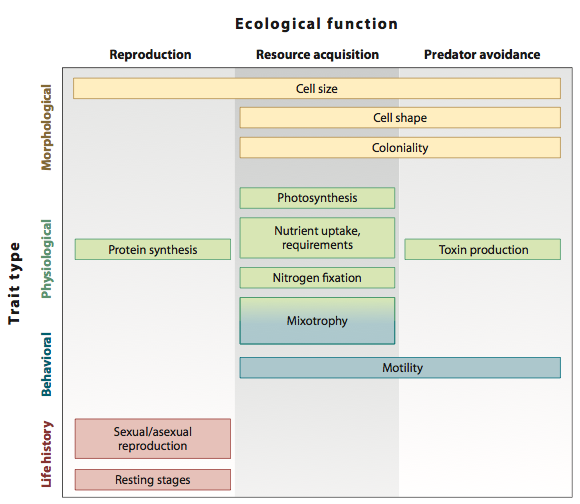
\includegraphics[width=0.7\linewidth]{./Chp1-Intro/Fig_litchman2008.png}
\caption[Scheme]{\small{Phytoplankton functional traits. Taken from \citet{Litchman2008}}}
\label{phytotrait}
\end{figure}

\subsection{Cell size a major trait to characterize phytoplankton community structure}
The cell size have a major influence on many eco-physiological processes, such as growth, photosynthesis, nutrient acquisition, sinking rates, grazing, population abundance and diversity \citep{Finkel2009a}. Plankton size varies across a wide range, from picoplankton ($<$2 $\mu$m) to macroplankton (200 to $<$2000 $\mu$m). Many of the processes related to size can be described using a simple power law function of $Size \propto aV^ b$, where $V$ is the cell volume or biomass. This simple function is an universal law in biology \citep{Platt1981}. For example, phytoplankton growth and intracellular concentrations of nutrients and carbon are negatively related to cell size \citep{Tang1995}. Suggesting that larger cells grow slowly. 

In a similar fashion one can determine the trade-off between size and metabolic processes. Previous studies measuring this interaction suggest that respiration rate increments with size \citep{Laws1975, Lopez-Urrutia2006} and photosynthetic rates, light absorption and pigment concentration decreases with size \citep{Ciotti2002,Finkel2004}. Suggesting that under light-limited conditions smaller cells are more efficient using the energy due to a stronger package effect on larger cells. However, this effect is masked under natural conditions due to the species assemblage of a community, in which each species (especially larger organisms) has specific strategies that help maintain higher metabolic rates under adverse conditions \citep{Maranon2009}. 

The nutrient uptake decreases with the size of the cell. But the advective transport of nutrients is enhanced by turbulence, sinking and swimming, which increases the flux of nutrients from the diffusive boundary layer favoring larger over small cells \citep{Kiorboe1993}. However, small phytoplankton could also benefit from the smaller surface to area relationship having a competitive advantage under low nutrient conditions.

Sinking velocity is also associated with size. This dynamics can be described by Stoke's law, predicting that sinking velocity increases with cell size \citep{Reynolds2006}. However, larger organisms such as diatoms, can regulate buoyancy by changing their density \citep{Reynolds2006}. 

Other characteristics of higher hierarchical levels can also be described using an allometric relationship of size such as the population density, interspecific interactions and diversity. The abundance of certain population ($Num.cells/L$) can then be described as a function of input and output of nutrients, based on the Droop model, to scale up to species abundance \citep{Irwin2006}. Irwin et. al. observations suggests that smaller cells are more abundant than larger organisms under limited nutrient conditions. 
Interspecific interactions, such as grazing, are also size-specific. Larger grazers feed on larger phytoplankton with a size ratio of 1:10 predator and prey \citep{Kiorboe1993}. This interspecific pressure governs the trade-off between size-related nutrient uptake and predation avoidance \citep{Thingstad2005,Naselli-Flores2007}. 

The diversity of a community ($Num.species /L$) is represented with a skewed log-normal distribution of the cell diameter, a mean cell diameter and a standard deviation on log scale. In this function the highest diversity occurs at values smaller than the median \citep{Irwin2006, Cermeno2008a, Finkel2009a}. Although, phytoplankton are widely distributed they do not show any large-scale diversity patterns across latitudinal scales and productivity gradients. The involved mechanisms for such a lack of pattern are: the high dispersal capabilities, the high patch connectivity, the chaotic biological interactions, the short generation times and the high frequency of environmental reset \citep{Cermeno2008}. The governing process over this trait in large scales appears to be non-equilibrium dynamics as early suggested by Hutchinson\citeyearpar {Hutchinson1961} in his plankton paradox tenet.

\section{Trait-based models of phytoplankton communities}
The so called, \textit{in silico} approach to study plankton communities is preceded by a history of breakthroughs of more than 70 years old \citep{Gentleman2002}. Early developments in plankton models were based on nowadays “simple” Lotka-Volterra predator-prey dynamics \citep{Fleming1939}. As advances in computational capabilities increased, models start to become more complex at point where now the typical nutrient-phytoplankton-zooplankton-detritus (NPZD) models are resolved for various zoo and pytho PFTs and over three-dimensional ocean circulation models. However, the increase parameterization of such a model came with the trade-off of increased uncertainty of many parameters. Thus, the challenge of developing a model is that it have to incorporate all the essential compartments and processes, but also be simple enough to be explained by \textit{in situ} and \textit{in vivo} observations with the few possible parameters \citep{Anderson2010}.

We started our discussion earlier on the difference between the trait and species type of perspective. The trait-based perspective to community ecology, offers a simpler and reliable framework for a simpler theoretical implementation. While the species-based would need a higher order of complexity to described mechanistically all the possible variation. Nowadays, computer and technical capabilities allow us to deal with this increased complexity, but it also difficult a wider applicability and interpretation of the model results.

The mechanistic description of traits and the cost and benefits of their implementation (i.e. trade-offs) allows to reduce the complexity of the models implementing specific metabolic rates based on the Dynamic Energy Budget theory \citep{Kooijman2009} and deriving a mechanistic trade-off function from the selected traits\citep{Merico2009}. See \citet{Follows2011} for a detail review on the topic.

For phytoplankton communities this approach could be implemented using a master trait, such as cell size, together with other traits such as the energy and nutrient allocation and the susceptibility of being grazed (edibility) \citep{Litchman2008,Follows2011}. Recent implementations of this modeling framework showed interesting results \citep{Bruggeman2007, Merico2009}, setting up new avenues of possibilities to explore. Trait-based models so far had been successful describing the community dynamics based on observations of a single trait and a fitness function describing the trade-offs with energy and resource allocation traits. In addition some models specify a top-down control setting up a fixed grazer compartment, and mortality rates for phyto- and zooplankton. Advances in this field should include a dynamic trait and trade-offs definitions for the grazer, for example. Further developments of \textit{in silico} studies of phytoplankton community size-structure will help us to understand mechanisms that drive natural variation under changing environmental conditions.

\section{Aims of the proposed PhD project}
The general aim of my PhD project is to study the processes that structure the phytoplankton community in the Atlantic Ocean, using a trait-based perspective. The specific aims during the course of the project are to:

\begin{itemize}
\item Develop a trait-based characterization of phytoplankton communities in contrasting regions of the Atlantic Ocean. 
%We are going to use an ocean basin dataset of the size fractionated chlrolophyll-a, together with data of the \textit{in situ} enviromental conditions, from the Atlantic Meridional Transect Program (AMT) (www.amt-uk.org) to study the patterns of phytoplankton community-size structure. Previous studies using this dataset, have been focus on the description of the ocurrence of the size fractions using information on just a few cruises \citep{Maranon2001}. With this analysis we atempt to extend the existing knowledge on phytoplankton community size-structure in the Atlantic Ocean using a larger dataset. Also we attempt to reconstruct the community size structure of phytoplankton relating the variation of the size classes with the prevailing environmental contidions, without any spatio-temporal consitrain. This work will also provied us the necesary information for contraining the further size-based model.

\item Implement a size-based model to understand the community composition in contrasting regions of the Atlantic Ocean.
\item Extend the proposed size-based model to incorporate a multi-trait mechanistic description based on the phytoplankton and the zooplankton size-structure.
\item Develop a paleo-reconstruction of phytoplankton communities using the proposed size-based model.
\end{itemize}
